% This template is used by DATS capstone students at the George Washington University in Washington, DC.
\documentclass{article}
\input{Auxiliary-Files/File_Setup}

\begin{document}
\begin{titlepage}
	\centering
	
\includegraphics[width=0.6\textwidth]{George-Washington-University-Seal-Logo.png}\par
	\vspace{2cm}
	{\scshape\LARGE Data Science Program\par}
	\vspace{1cm}
	{\scshape\Large Capstone Report - Spring 2026\par}
	\vfill
	
	%%%% PROJECT TITLE
	{\huge\bfseries Civil War Recovery in Internationalized and \\Non-Internationalized Contexts\par}
	\vfill
	
	%%%% AUTHOR(S)
	{\Large\itshape Hazel Lutz}\par
	\vspace{1.5cm}

    \vfill
    \emph{A capstone presented in fulfillment of the requirements \\for the degree of Bachelor's of Science in Data Science}

	\vfill
	supervised by\par
	%%%% SUPERVISOR(S)
	Prof. Sushovan Majhi

	\vfill
% Bottom of the page
\end{titlepage}

\newpage

\begin{preface}
        This is the final result of my research for my Data Science Capstone at The George Washington University, and in many ways, the final result of my overall trajectory as an undergraduate. It was profoundly educational on the translation of theory to quantitative practice and the limitations thereof. It was also my most ambitious project at the undergraduate level: though I had done quantitative political science research prior, it used more available data that was far easier to work with. From start to finish, this project required a lot of evaluation of political science literature and methodological studies -- I had only heard of qualitative comparative analysis prior to this, and I could not resist the challenge of learning about this methodology and practicing it based primarily on textbooks and articles rather than step-by-step instructor direction, as I had done prior for methods like frequentist and Bayesian regression. I look forward to employing what I've learned here as I go on to graduate studies in the coming weeks.

        The project was inspired in large part by the end of the Syrian civil war, as discussed in the introduction; the complex circumstances of the course it ran and the lack of quantitative data due to its violence and instability forced my attention to the staggering human suffering caused by governments seeking only to improve their domestic circumstances as well as an emerging gap that could be studied by political science. This study seeks to begin the work of filling that gap in. Internationalized civil wars, like Syria's, have been considered by pundits and scholars alike to be more complicated than non-internationalized in a number of ways; this article quantitatively evaluates that assertion and applies it to the success of civil war recovery. Theoretical implications largely stem from the furthering of that distinction and quantitative considerations that should be made, and policy implications are built on the application of that theory -- notably, the caution that should be taken when extending conclusions from non-internationalized civil wars to internationalized ones. 
\end{preface}

\vspace{1cm}

\begin{acknowledgements}
I would like to thank Georgia Semenzato for her constant support throughout my years at The George Washington University.
\end{acknowledgements}

\newpage


\begin{abstract}
        Internationalized civil wars have been found to be uniquely complicated when they occur, but few evaluate the importance of this distinction once the conflict has ended. This study evaluates two questions pertaining to civil war recovery: first, do commonly-cited features of civil war outbreak and recovery function as isolated necessities for recovery in internationalized civil wars specifically, and second, how do internationalized and non-internationalized civil wars differ in the sufficient combinations of conditions for recovery? Using qualitative comparative analysis and data from the Correlates of War project from 1990-2014, V-Dem, the World Bank, and others, this study finds evidence that suggests that, for the time period in question, individual factors are inadequate as necessities for recovery at the 0.9 inclusion level and combinations of conditions should instead be used and that internationalized civil war recovery cannot be explained as easily as non-internationalized cases and requires more specific conditions. QCA on internationalized cases failed to significantly explain over half of the successful recovery cases, while QCA on non-internationalized ones explained almost 80\% of them. Future studies may benefit on elaborating on nuances concealed by quantitative study through close case studies or by testing a broader number of variables through methods like regression, though both should be attentive to the results found here when doing so.
\end{abstract}
\vspace{1cm}

\begin{keywords}
\centering
        \textbf{Capstone; data science; GWU; civil wars; civil war recovery; post-conflict; qualitative comparative analysis; internationalized civil wars}
\end{keywords}

\newpage



\doublespacing
\tableofcontents
\singlespacing

\newpage

\doublespacing

\section{Introduction}
After over a decade, the Syrian civil war came to a tentative close in December of 2024, when rebel leader Ahmed al-Sharaa and his rebel group Hay’at Tahrir al-Sham stormed Syria’s capital, leading to former dictator Bashar al-Assad’s flight from the city. In the year since, the new Syrian government has engaged in numerous measures to re-establish sovereignty and legitimacy in a country still fractured by numerous rebel groups and regime elements, each with a degree of external support. Continued conflict between the current government and other groups with claims to sovereignty, such as the Kurdish-led Syrian Democratic Forces (SDF) after a breakdown in transition negotiations and the Israeli-backed Druze in the southwest, threatened to destabilize reconstruction efforts and cause a resurgence of war. These turbulent forces have begun to settle once more ~\cite{ap-us-withdrawal} ~\cite{ap-syria-corridor}, though whether this is settling down into a lasting peace or merely a brief respite from war remains to be seen.

Syria's civil war was long, bloody, and complicated; though early estimates of the war's length believed it would be fleeting, by a few years in, policy circles alike realized this would not be the case ~\cite{tabler-fa}. Political science research, such as Sharif's article in 2017 ~\cite{sharif}, find the cause of this poor prediction of length was the consequence not of poor methodology, but of a fundamental misunderstanding of the conflict that failed to recognize the impact of a splintered opposition created in part by staggering amounts of foreign involvement. "Internationalized" civil wars are large-scale intra-state conflicts in which external actors -- such as global powers like the US, China, and Russia, or regional poles such as Saudi Arabia, Iran, and the UAE in the Middle East -- become involved in combat through aiding one or more parties to the conflict by providing money, weapons, training, or direct support from their military. These conflicts more broadly have been found to be distinct from non-internationalized civil wars in having unique obstructions to successful negotiation ~\cite{kane} and further fragmenting opposition powers during the conflict ~\cite{eleftheriadou}. However, comparatively little research has been done on the lasting impacts of this to a post-conflict environment. This gap, if explored, could provide key insights into the needs of recovering states in internationalized civil wars, as well as provide reason to further distinguish between internationalized and non-internationalized civil wars in quantitative political science research. 

To begin to fill in this gap, this study will analyze the necessary and sufficient conditions for recovery for civil wars from 1990-2014 in internationalized and non-internationalized cases. Here, internationalization is defined strictly as the direct supply of troops by a state external to the conflict to support one side of it ~\cite{sarkees}, and recovery is defined as the permanent decrease of fatalities to non-war levels in line with the standard definition of below 1000 deaths in a 12-month period ~\cite{cow} ~\cite{caplan}. Two guiding questions related to civil war recovery from 1990-2014 were evaluated, which was a period in which civil wars became an international focus but before a later spike in internationalized civil wars ~\cite{bellamy}. First, how do commonly-cited individual factors in civil war recovery fare as necessities for recovery when considering only internationalized cases? And second, how do the same sets of conditions for recovery differ between internationalized and non-internationalized civil wars? Both of these questions were answered with qualitative comparative analysis (QCA), which evaluates whether conditions are necessary, sufficient, or neither for an outcome in question -- here, whether or not conflicts returned to the level of a war. By performing QCA on an individual-level for a number of conditions, this study finds no variables that are independently necessary for successful recovery, indicating the importance of studying the convergence of multiple conditions. As for the latter, QCA was performed on the combination of four conditions and compared between datasets, which found that internationalized cases were more poorly explained and required more specific combinations of conditions than non-internationalized cases, suggesting that the increased complexity of internationalized civil wars extends to recovery and that lessons learned from non-internationalized civil wars should not be extended to internationalized ones. These results should guide further research, in both large-$n$ studies and smaller case studies, and suggest the importance of specific, local-level knowledge in internationalized civil war recovery. The specific combinations of conditions found to be significant, though, should not be directly considered without further research on them: QCA here does not seek to "solve" civil war recovery and, given the few variables used and cases analyzed, should not be considered exhaustive or generalized beyond the years studied. That is, the scope of this includes only determining the extent of the distinction between internationalized and non-internationalized civil wars; the scope is not to find all potential causal factors, and interpreting it as such may neglect other explanations.

Section 2 will elaborate on previous literature on civil wars and civil war recovery to guide what variables will be selected for analysis, as well as build the theoretical ground on which this research is done. Section 3 will discuss the methodology used -- namely, qualitative comparative analysis; this includes the history of the methodology, the mathematical basis of it, software used, what results to expect, and how they will be evaluated. Section 4 will detail how data was sourced, the variables used, and how these variables were calibrated for qualitative comparative analysis. Section 5 will present the results of the analysis and briefly contextualize how statistical results should be interpreted. Section 6 will elaborate on what the results indicate more broadly for both an academic and policy audience (and perhaps more importantly what they do not indicate), and relate these to initial research question. Section 7 will conclude by summarizing the research performed and provide avenues for future research alongside stating the limitations of this research and what it should not be interpreted to indicate.


\section{Literature Review}
\subsection{Defining civil war, internationalization, and recovery}
To guide the rest of this study, it is worth defining key terms here. There is substantial debate over what qualifies as a civil war, an internationalized civil war, and what successful recovery means; therefore, any conclusions about these factors will be contingent on the definitions used. The definitions adopted for the analysis done below will require moderating theoretical positions found in the sources analyzed below with the quantitative data made available. Decisions made on that front will be carefully justified using literature from both data-collection organizations as well as academic literature, and limitations resulting from this should be addressed.

First, the object of study is a civil war. Sambanis's key work on defining civil wars in political science research begins with the "deceptively straightforward" definition used by Small and Singer in 1982: "any armed conflict that involves (a) military action internal to the metropole, (b) the active participation of the national government, and (c) effective resistance by both sides" ~\cite{sambanis}~\cite{small-and-singer}. That is, a civil war is one that is conducted within an existing state's borders, the ruling government is one of the parties engaged in fighting, and state violence is "sustained and reciprocated", usually requiring more than 1000 deaths ~\cite{sambanis}. The false simplicity, though, comes from difficulty applying it to edge cases where the state hires proxy fighters, to wars for independence within existing states, issues with reporting deaths, and determining when civil wars end. Sambanis's study, through performing regression with multiple different datasets based on different criteria for civil wars, finds that sign, magnitude, and significance of regression coefficients can vary drastically for some variables -- though primarily it cautions against predictive modeling on civil war onset and termination based on commonly theorized risk factors like low GDP, population growth, and ethnic heterogeneity ~\cite{sambanis}. The questions this study seeks to analyze are primarily descriptive, though the same concerns are worth noting. 

An internationalized civil war, at its loosest definition, is one in which a state external to the one in which conflict occurs provides material support to either the existing government or one of the rebel groups; this includes direct support with troops, hiring of mercenaries, supplying weapons, or perhaps even provision of financial support ~\cite{bellamy}~\cite{kane}. Clearly, this muddies the picture of the clear distinction between interstate and intrastate wars as outlined by Small and Singer. Internationalization is also liable to make intrastate conflicts quickly spill over into regional war complexes characterized by conflict within and between neighboring countries against at least one state or perhaps one another ~\cite{gersovitz}. A broad definition of a civil war that includes such cases may lead to useful results (and could become increasingly relevant as internationalized wars become more common ~\cite{bellamy}, but this would surely complicate quantitative analysis. For this reason, popular conflict datasets usually use strict definitions for both civil wars and internationalization.

One of the most common datasets on civil wars is the Armed Conflict Dataset by the Uppsala Conflict Data Program and the International Peace Research Institute; this classifies a "war" as a conflict involving over 1000 deaths in each calendar year and intrastate wars being ones between a government and at least one rebel group. These become internationalized intrastate wars when "there is involvement of foreign governments with troops" ~\cite{ucdp}. Under the typology made by Bellamy in 2023, this falls into direct rather than indirect support, which involves material aid without the use of external troops ~\cite{bellamy}. Similarly, the Correlates of War project's Intra-State Wars database requires a minimum of 1000 fatalities within a 12-month period, and explicitly cites Small and Singer's other criteria ~\cite{sarkees}. An internationalized civil war in their dataset similarly involves the direct intervention of an external state by either committing over 1000 troops or suffering 100 deaths, but they also require that the external state does not do "the bulk of the fighting" ~\cite{sarkees}. The Correlates of War dataset, then, appears to be more strict, although it contains less recent data ~\cite{cow}.

Recovery from war, too, can be defined in a broad number of ways. Theoretically-useful but quantitatively challenging definitions are worth noting for contextualizing this study's results to broader theoretical practice: for instance, the process of peacebuilding as used by Erinosho in 2020 involves the long-term creation of institutions to undergo the process of creating peace and maintaining it, both culturally and politically ~\cite{erinosho}. Caplan in 2019 defines many conceptions of peace from "minimal" to "maximal". The former is primarily a negative definition based on the absence of armed conflict and may not reflect the sort of enduring peace defined above by Erinosho; unfortunately, this tends to be the standard with quantitative datasets precisely because "maximal" definitions are more positive, unspecific, and have more nuance ~\cite{caplan}. To achieve the latter, manual coding would likely be necessary, alongside detailed local-level information about post-war institutions and enough time to be able to adequately reflect on it, and further, such idealistic definitions can frequently entail normative evaluations about what is desirable to the author. This may include the creation or improvement of democratic institutions, a more powerful and centralized state, changes to the economic system, and more -- many of which might be instead used as independent variables in quantitative analysis. Due to all of these constraints, a minimal definition was necessary for the study done here. 

\subsection{Relevant variables for outbreak and recovery from civil war}
Many studies find relevant factors, through either quantitative or qualitative methods, that influence the outbreak of civil war and successful recovery from it; many agree, some disagree. One of the most cited articles on the causes of civil wars, and emblematic of the disagreement in this object of study, is Dixon's article in 2009 which overviews 46 different studies with over 200 independent variables to analyze agreement and disagreement between them. General categories are demography, geography, resource wealth, economic variables, government type, and history. The variables for which there was a substantial amount of agreement are too many to name, and in-line with the scale of this study, existing, publicly available data will be prioritized: this includes economic growth, oil exports, and democracy measures ~\cite{dixon}.

More specific studies, such as by Basedau and Richter's in 2013, tend to narrow in on specific categories of variables and gauge interaction. They consider many oil-related variables using qualitative comparative analysis, including resource wealth, and find that several oil-related conditions are interdependent and influential in creating the "resource curse", in which extreme abundance and dependence creates political and economic stakes so drastic that contestation over power is less likely to be peaceful or stable ~\cite{basedau}. However, contrary to Dixon's conclusions, oil-related measures considered in isolation were not enough. High dependence and low democracy was heavily related to the outbreak of civil war, and low dependence with high democracy had the opposite effect. This work also provides general guidance for the scope of QCA as a methodology. It does not seek to be fully predictive, as Basedau and Richter consider only a few, heavily related variables; instead, it contributes to existing theory and contributes to the considerations made by broader studies or comparative analyses. 

One notable feature of the time period studied here -- a decision made largely for practical reasons, and partially for theoretical ones -- is the role of the UN. Starting in the wake of the Cold War, the UN under the guidance of Secretary General Boutros Boutros-Ghali began to consider civil wars, post-conflict peacebuilding, and liberal democratic theories more seriously. Intra-state wars were believed to be worth intervention to the same degree as inter-state wars due to their ability to destabilize other countries and spread across borders ~\cite{hozic}. In general, this led to more UN peacekeeping operations to seek to stabilize countries after civil wars and negotiate cease-fires as well as seeking to influence the resulting regime's governmental form. Ultimately, this contributed to the norm of intervention that only grew more common and consequential after the US's war on terror ~\cite{hozic}, with some scholars arguing that this UN trend may have worsened international stability in some cases ~\cite{bayrasli-fa}. Considering these theoretical discussions and case studies, then, the interaction between democracy, peacekeeping operations, and other material conditions may be an area that should be further explored.

\section{Methodology}
\subsection{Fundamentals of Qualitative Comparative Analysis}
The methodology used to answer the last two questions will be qualitative comparative analysis (QCA), a social scientific technique described by Ragin in 1987 that identifies necessary and sufficient conditions for a desired outcome: in this case, success of recovery after a civil war. This methodology was selected for some theoretical reasons as well as reasons pertaining to the data collected. For the former, qualitative comparative analysis is primarily used to identify both necessary conditions for the defined outcome variable as well as numerous sufficient \textit{combinations} of conditions. This is an increasingly popular methodology for social science because of its utility in situations with causal complexity. This causal complexity is characterized by the potential non-significance of isolated variables alone, the possibility for multiple pathways to the same outcome, and the potential for the outcome or lack of it (e.g., success/failure of recovery) to have different explanations ~\cite{mello}. For instance, oil rents may be a significant condition for the recurrence of conflict in non-democratic states, as contestation over such a large source of GDP may lead to the resurgence of violent conflict, but in democratic states such a threat may not be as severe. But perhaps neither of those two variables are necessary for recovery when there is a UN peacekeeping operation on the ground and there were not enough deaths to create a lasting national scar. As for the datasets it is most useful for, while regression may require a large number of observations to be significant, qualitative comparative analysis can provide significant insight with as few as 20 cases ~\cite{mello}. 

The fundamentals of the methodology are heavily based on mathematical set theory; this considers whether or not a particular case is included or excluded from a collection based on a variable (for example, whether or not a UN peacekeeping mission was present), with that case being assigned a 1 on that condition if it is included and a 0 if excluded. Where the line between inclusion and exclusion is drawn is important and is where the qualitative focus comes in: qualitative comparative analysis determines the significance of qualitative differences based on quantitative inputs. One explanatory example is that when water goes from 1C to -1C, the quantitative shift of 2C indicates a qualitative change that one might be interested in, namely freezing. However, the same quantitative shift from -1C to -3C causes no further qualitative change, since it remains frozen, and is therefore irrelevant if freezing is a variable of interest ~\cite{mello}. Previous relevant research using QCA follows similar logic: for instance, Basedau and Richter use a cutoff for oil rents as 0.15 for the qualitative change of oil dependence; that is, if 15\% of the GDP of a country is from oil exports, then it will be considered oil dependent for the purposes of explaining the incidence of civil war ~\cite{basedau}. So, if a country increases their oil dependence from 0.01 to 0.08, this will not make their economy dependent on oil, but if another increases it from 0.11 to 0.18, it will be considered dependent and therefore potentially increase its risk of having a civil war, though this risk is not further increased if it goes from 0.18 to 0.25. This, alongside other criteria, are used to create a truth table of combinations of inclusion and exclusion for all the conditions included, where each case falls into one row representing one combination of conditions.

The aforementioned examples all involve crisp sets, in which a case is either firmly included or excluded. However, this may fail to capture all the complexities of the circumstance in question: for example, perhaps a change in oil dependence from 0.01 to 0.08 has some consequence, though it may be more slight than the change from 0.11 to 0.18. To deal with this, fuzzy sets have become increasingly popular for qualitative comparative analysis for instances where such a clear division is difficult or less useful ~\cite{mello}. As the name implies, this involves "fuzzy" criteria for set membership, where exclusion and inclusion are placed on a scale from zero to one. This requires "calibration", which determines whether or not a certain case is fully included (1), fully excluded (0), at the crossover point (0.5), or somewhere in between. Calibration requires determining what qualifies as each of these three primary cases, where the crossover point can be especially important for being the "point of maximum ambiguity" ~\cite{ragin}. Cases are then placed on a logistic curve on this scale, where the crossover point has the steepest slope. Therefore, changes in that midpoint are most consequential for inclusion or exclusion. Continuing the crisp-set example, one should make the crossover point for oil rents as \% of GDP be 0.15, since this will make crossing that threshold very important and changes higher or lower less consequential. 

QCA, however, is limited by the relatively few number of conditions that can be effectively analyzed with it: while methodologies like linear regression are capable of handling vast numbers of potential regressors related to the studied outcome, the use of truth tables for crisp-set QCA means that, given $k$ conditions, the number of rows in the truth table is $2^k$ (since there must be one row for each combination of boolean true/false conditions). Given the few number of cases QCA is designed to study, this means that, given a dataset with 35 different cases, only 5 conditions should be analyzed since the truth table would have $2^5$, or $32$, rows; fuzzy-set QCA makes this requirement even more important, as inclusion and exclusion is no longer binary. The scope of this study therefore implies different conclusions from a study that involves regression, for instance. It does not seek to provide all, or even a significant amount, of the explanatory factors for the success or failure of civil war recovery: instead, it quantitatively evaluates the relevance of the distinction between internationalized and non-internationalized civil wars. It is the domain of future research to fully elaborate on the distinctions that matter. In light of the limited number of variables used, then, "QCA studies should always provide a careful \textit{justification} for their selection of conditions" ~\cite{mello}.

\subsection{Evaluating results of QCA}
The analysis itself requires determining the necessity of conditions, defined as whenever the outcome occurs, those conditions are present (in set-theoretic language, the set of cases with the desired outcome, referred here as $Y$, are a subset of the set of cases in which those conditions are present, referred here as $X$). The truth table is then analyzed by QCA software to determine the confluences of factors that lead to the desired outcome and removing the factors whose presence or absence does not affect the outcome. 

When evaluating necessity of conditions, the statistics generated in this analysis are "inclusion" or "consistency", "coverage", and "relevance of necessity". Consistency measures how much of the set of cases with the desired outcome is in actuality a subset of the set of the cases in which that condition is present. Defined mathematically, let $f_X(i):\mathbb{N}\to[0,1]$ be a function that maps case $i$ to its fuzzy score for inclusion in the set $X$ for one condition in question, and $f_Y(i):\mathbb{N}\to\{0,1\}$ map case $i$ to its crisp score for inclusion in the set $Y$ for the binary outcome of successful or unsuccessful recovery. Then the inclusion score for necessity of the condition $X$ for outcome $Y$ is
$$inclN=\frac{\sum_{i=1}^n\min(f_X(i),f_Y(i))}{\sum_{i=1}^n f_Y(i)}.$$
Since $Y$ is a crisp set, if case $i$ is not in the outcome set, then that term in the sum will be zero, and if case $i$ is in the outcome set, then the term in the sum will be case $i$'s fuzzy score for condition $X$; all of this is divided by the number of cases included in the outcome set ~\cite{dusa-book}. $inclN$'s codomain is then between $0$ and $1$, and a consistency of 0.9 is the recommended minimum to find a strong set relation of necessity between the outcome set and condition set (though weaker relations can still be considered relevant). Coverage measures to what extent a condition is present overall compared to the outcome; if a condition covers all cases, then though the outcome set is a subset of the condition set, so is the complement of the outcome set. Therefore, though it would be considered highly necessary by the consistency measure, practically, it is irrelevant. This is similar to consistency, varying only in reversing in which direction the subset relation goes. Therefore, using the same function and set definitions as above, we have
$$covN=\frac{\sum_{i=1}^n\min(f_X(i),f_Y(i))}{\sum_{i=1}^n f_X(i)}.$$ 
A coverage above $0.5$ is considered adequate for a condition to be considered non-trivial. A common third metric is "relevance of necessity" which measures to what degree the condition variable is constant, measuring triviality in a way not always caught by coverage. This is given by
$$RoN=\frac{\sum_{i=1}^n(1-f_X(i))}{\sum_{i=1}^n(1-\min(f_X(i),f_Y(i)))},$$
and a score of above 0.5 is also considered sufficient to consider a condition significant ~\cite{mello}.

As for sufficient conditions, which are used for more complex models where there are multiple pathways to the same outcome, only consistency/inclusion and coverage are used. The outputs of a sufficiency analysis will be multiple different combinations of conditions, each of which partially explains the outcome, the combination of which creates a significant model. Because inclusion seeks to gauge to what extent the condition set $X$ is contained within the outcome set $Y$, or $X\subseteq Y$, compared to the number of cases in which that set of conditions is present, inclusion for sufficiency is given by
$$inclS=\frac{\sum_{i=1}^n\min(f_X(i),f_Y(i))}{\sum_{i=1}^n f_X(i)}.$$

Likewise, coverage seeks to measure how much of the outcome set $Y$ is explained by the condition set $X$ compared to the entire outcome set; that is, $Y\subseteq X$. Therefore,
$$covS=\frac{\sum_{i=1}^n\min(f_X(i),f_Y(i))}{\sum_{i=1}^n f_Y(i)}.$$
$InclS$ of the overall model and each combination of conditions should generally be greater than 0.8 to be considered significant, and though $covS$ for each row of the truth table tends to be lower, the overall model's coverage should be similar to that of necessary condition analysis ~\cite{pappas}. Since this does not consider the necessity relation, $RoN$ is not measured.

These statistics, as well as the conditions or combinations of conditions that meet the benchmarks specified above, were generated using the \texttt{qca} package in R; for necessity analysis, this involved calibrating the variables and using the \texttt{pof()} function, and for sufficiency analysis, calibrated variables were turned into a truth table via \texttt{truthTable}, and then the combinations of conditions were reduced to include as few conditions as necessary to remain significant to the model using \texttt{minimize()} ~\cite{dusa-pkg}. 

\section{Variables and Datasets}
\subsection{Sources and variables}
The cases of civil wars were sourced from the Correlates of War's Intra-State War v5.1 database ~\cite{cow}. This dataset contains all of the downsides mentioned in the literature review -- primarily, that it contains a strict definition of internationalization and it considers "peace" to be when the total number of fatalities drops below 1000 for a 12 month period. The latter is represented in the dataset by multiple start and and years in the same row (each row representing one civil war). "Successful recovery", then, has the same minimal definition described by Caplan, which is merely that conflict has calmed down, though it may not have ceased entirely ~\cite{caplan}. Though not a robust definition of peace by any measure, it is in line with the scale of this study, and the definition should be considered when drawing conclusions.

These civil wars were split into two datasets based on whether or not it was considered internationalized by the Intra-State War database (which contains a binary internationalization column) and separated into episodes of conflict between each start and end year. If there was a subsequent start year in the same conflict -- i.e., fatality levels returned to war-like levels -- recovery was considered failed. If that episode was the last end year for that civil war, then recovery was considered successful. The last year included in the dataset was 2014 -- a potentially changing character of internationalized civil wars around this year makes it also an adequate cutoff for theoretical reasons as well ~\cite{bellamy}. 1990 was used as the earliest year included to coincide with the eventual end of the Cold War and the changing role of the UN ~\cite{hozic}. 

QCA was performed on a number of the aforementioned factors. These include economic improvement measured as change in GDP per capita (measured in USD); increase in participatory democracy from V-Dem v16's zero-to-one scale; oil rents/exports as a \% of GDP from the World Bank, which is updated regularly; the number of deaths during each conflict episode from the Intra-State War v5.1 database; and the presence or absence of a UN peacekeeping operation (PKO), which was hand coded. Calibration and the eventual full analysis were done using R's \texttt{qca} package. All but whether or not there was a UN PKO were calibrated as fuzzy sets; the criteria for the calibration and data sources are summarized in Table~\ref{tab:qca_conditions}. All of these variables were merged into one dataset each for internationalized and non-internationalized cases through matching country-year pairs.

\begin{table}[ht]
    \centering
    \small
    \begin{tabular}{p{4cm} p{2.5cm} p{1.5cm} p{3.5cm}}
        \hline
        \multicolumn{4}{c}{QCA Condition Summary} \\
        \hline
        Variable and Abbreviation & Source & Set Type & Calibration (exclusion, crossover, inclusion) \\
        \hline
        Change in GDP per capita ($\Delta GDPPC$) & ~\cite{fariss} [v4] & Fuzzy & -0.04, 0.1, 0.3 \\
        Change in participatory democracy ($\Delta PD$) & ~\cite{vdem} [v16] & Fuzzy & -0.001, 0.0015, 0.03 \\
        Oil rents (\% of GDP) ($OR$) & ~\cite{vdem} & Fuzzy & 0, 0.15, 0.35 \\
        Deaths ($TD$) & ~\cite{cow} [v5.1] & Fuzzy & 1000, 8000, 30000 \\
        UN PKO ($PKO$) & ~\cite{un-pko-list} & Crisp & Present $\to$ 1,  Absent $\to$ 0 \\
        \hline
    \end{tabular}
    \caption{Variables, sources, set type, and calibration criteria.}
    \label{tab:qca_conditions}
\end{table}

\subsection{Resulting datasets}
The total number of rows -- that is, episodes of conflict considered here -- was $106$, $43$ of which were internationalized conflicts and $63$ of which were non-internationalized. However, after removing rows in which missing values were present (generally due to lack of information on the change in participatory democracy or oil rents), there were only $26$ cases of internationalized conflicts and $35$ cases of non-internationalized conflicts for a total of $61$ cases studied. In line with the specifications of qualitative comparative analysis, this means that approximately $4$ variables should be used for sufficiency modeling. Calibration as a part of qualitative comparative analysis deals with other irregularities in the data, such as outliers, by focusing on the quantitative threshold at which qualitative change takes place and nothing else.

Calibration graphs are also included in the \hyperref[appendix]{Appendix} to show the distribution of cases across the fuzzy-set calibration and number of cases for each inclusion or exclusion in the crisp-set UN PKO condition. Fuzzy membership scores were determined by the \texttt{calibrate()} function and sit on a $[0,1]$ scale, and cases were sorted to demonstrate the logistic curve; index in that sorted list is shown in these figures. Goals in calibration were, first, to follow theoretical best-practices for crossover points should be (where applicable), and second, to spread points across the logistic distribution second to have high variation in set membership. Adjustment to improve the distribution within the theoretical bounds were tested without significant changes to either resulting truth tables or the differences between internationalized and non-internationalized ones. One distribution worth noting especially is Figure~\ref{fig:oil-rents}, which has very few cases not at zero or one -- oil dependence was very bimodal. Crisp-set methods would capture a large part of the variation here and is therefore certainly viable, but nothing is lost in this study by making it fuzzy-set. All of the other fuzzy variables (Figure~\ref{fig:gdppc}, Figure~\ref{fig:partipdem-dif}, Figure~\ref{fig:deaths}) generally follow a clean logistic distribution, and Figure~\ref{fig:un-pko} shows that, though there are more cases without a UN peacekeeping operation, there are certainly enough of each to draw conclusions.

The Intra-State Wars database was accessed most recently on March 23rd, 2026, while all others were accessed on April 27th, 2026. The final data collected can be found in the GitHub repository \href{https://github.com/GW-datasci/26-spring-LUTZ-H}{here}; cleaned datasets and original sources are found in the \texttt{data} folder, and running the code in \texttt{code/qca.Rmd} will reproduce the following results. Though historical data is not likely to be updated further, data for later years may be added, though these will not impact the local datasets; additionally, all of the \texttt{qca} functions are deterministic and do not include randomness, so all results are perfectly reproducible without a particular seed. 

% include ethics subsection, regarding data collection, biases, data licensing, include decision made regarding ethics
\section{Results}
\subsection{Necessity of individual variables}
This section addresses the first research question: do commonly-cited individual variables function as conditions for the reduction of conflict in civil wars? The results of the individual-variable necessity analysis done in R are shown in Table~\ref{tab:necessity-results}. Included in this table are one row for each condition analyzed, the $inclN$ score, the $RoN$, and the $covN$.

\begin{table}[ht]
    \centering
    \small
    \begin{tabular}{p{3cm} p{1.5cm} p{1.5cm} p{1.5cm}}
        \hline
        \multicolumn{4}{c}{Necessity of Individual Variables in Internationalized Cases} \\
        \hline
        Condition & inclN & RoN & covN \\
        \hline
        Change in GDP per capita & 0.390 & 0.885 & 0.763 \\
        Change in participatory democracy score & 0.443 & 0.856 & 0.755 \\
        Oil rents (\% of GDP) & 0.553 & 0.801 & 0.757 \\
        Number of deaths & 0.394 & 0.894 & 0.779 \\
        UN PKO & 0.444 & 0.889 & 0.800 \\
        \hline
    \end{tabular}
    \caption{Results of QCA on individual variables in internationalized civil wars.}
    \label{tab:necessity-results}
\end{table}

Notably, the highest individual-level inclusion score was for oil rents. But considering the significance testing done by $inclN$ and how not even oil rents broke the significance threshold of 0.9, oil rents is not a significant necessity for internationalized civil war recovery despite its adequate $covN$ and $RoN$. In fact, none of these conditions are alone significant necessities for recovery, since none meet the $inclN$ threshold. As previously mentioned, the number of rows in the internationalized civil war dataset were enough to include only 4 variables for the sufficiency analysis with combinations of conditions. Because the change in GDP per capita had the lowest consistency, this variable will be excluded for that analysis. Since the scope of the sufficiency analysis is not to draw broad conclusions about sufficient conditions for conflict resolution for both internationalized and non-internationalized cases but rather to note differences between them, the exclusion of this factor specifically does very little to hamper the results drawn. 

\subsection{Sufficient conditions between internationalized and non-internationalized cases}
This section addresses the second research question: how do the sufficient conditions for recovery differ between internationalized and non-internationalized civil wars? Through constructing the truth tables for each dataset -- internationalized and non-internationalized -- based on change in participatory democracy, oil rents as a \% of GDP, fatalities during conflict, and the presence of a UN PKO, the $inclS$ and $covS$ scores were calculated. If multiple models on pathways to successful recovery were generated, the overall consistency and coverage are also given. As discussed in the methodology section, the individual model terms' $covS$ need not be high (in line with the utility of QCA for finding multiple pathways to the same outcome), but the overall model should have a coverage of above 0.5. The higher the coverage is, the more cases are explained by the model generated. In each table, $\sim$ before a variable indicates an inverse relation: for example, $\sim\Delta PD$ indicates a decrease in participatory democracy scores, as measured by V-Dem. The cells under the columns labeled (M1) and (M2) indicate unique coverage -- or what proportion of cases covered by that term are uniquely explained by it and no other term in the model -- where an empty cell indicates that that term was not in the model. Unique coverage can be useful in some studies, but is not important for answering the questions above, so the overall unique coverage scores were not included, and the individual-model unique coverage scores are shown only to demonstrate when terms are not in the model.

\begin{table}[ht]
    \centering
    \small
    \begin{tabular}{p{5cm} p{1.5cm} p{1.5cm}}
        \hline
        \multicolumn{3}{c}{Sufficient conditions for recovery in internationalized civil wars} \\
        \hline
        Conditions & inclS & covS \\
        \hline
        $\Delta PD + OR + TD$ & 0.816 & 0.188  \\
        $\Delta PD + TD + \sim PKO$ & 0.873 & 0.108  \\
        $OR + TD + \sim PKO$ & 0.878 & 0.160  \\
        $\sim\Delta PD + OR + \sim TD + PKO$ & 0.813 & 0.124  \\
        $\Delta PD + \sim OR + \sim TD + PKO$ & 0.935 & 0.086  \\
        \hline
        (M1) & 0.891 & 0.465 \\
        \hline
    \end{tabular}
    \caption{Results of QCA on combinations of conditions in internationalized civil wars.}
    \label{tab:sufficiency-intl}
\end{table}

First, for Table~\ref{tab:sufficiency-intl}, there is only one model present, which contains five terms, all with an $inclS$ above the threshold of 0.8, for an overall model consistency of 0.891. This indicates that the model and its terms do significantly explain the cases that fit those criteria. However, it worth noting is that each of the terms in the model have a relatively low coverage -- all less than 0.2 -- and that the model coverage is less than 0.5. Therefore, there are still a large number of cases whose outcome was \textit{not} explained by this model, and the model failed significance testing to explain all cases of recovery. Additionally, all terms of the model include at least three of the four conditions, and two of them include all four: that is, the sufficient conditions for recovery in internationalized civil wars are very specific, and despite that specificity, relatively few cases ended up being explained.


\begin{table}[ht]
    \centering
    \small
    \begin{tabular}{p{5cm} p{1.5cm} p{1.5cm} p{1.5cm} p{1.5cm}}
        \hline
        \multicolumn{5}{c}{Sufficient conditions for recovery in non-internationalized civil wars} \\
        \hline
        Conditions & inclS & covS & (M1) & (M2) \\
        \hline
        $\Delta PD + \sim TD$ & 0.973 & 0.231 & 0.074 & 0.032 \\
        $OR + \sim PKO$ & 0.882 & 0.277 & 0.073 & 0.098 \\[6pt]
        $\sim TD + \sim PKO$ & 0.862 & 0.481 & 0.243 & 0.243 \\
        \hline
        $\sim\Delta PD + OR + TD$ & 0.937 & 0.186 & 0.070 & \\
        $\sim\Delta PD + TD + PKO$ & 1.000 & 0.105 & & 0.090\\
        $\Delta PD + \sim OR + PKO$ & 1.000 & 0.082 & & 0.027\\
        $\sim OR + TD + PKO$ & 1.000 & 0.058 & 0.042 &\\
        \hline
        (M1) & 0.901 & 0.788 & & \\
        (M2) & 0.901 & 0.790 & & \\
        \hline
    \end{tabular}
    \caption{Results of QCA on combinations of conditions in non-internationalized civil wars.}
    \label{tab:sufficiency-nonintl}
\end{table}

By comparison, Table~\ref{tab:sufficiency-nonintl} for the non-internationalized cases is much simpler despite two models being present, and both models have an $inclS$ of 0.901 -- above the required threshold, and comparable to the internationalized cases. Each model also has five terms, with model one and model two having coverages of 0.788 and 0.790, respectively. Many more cases were explained in the non-internationalized model than the internationalized one: while only 46.5\% (less than half) of successful recoveries were explained by the internationalized civil war model, most of the successful recoveries in the non-internationalized case were explained by the models -- approximately 79\% each. Furthermore, while the coverage of each term in the internationalized model was relatively low, the three terms shared by both models had coverages above 0.2, with one covering almost half of all successful recoveries. All three of these terms additionally only used two of the conditions present, and therefore are notably less specific. Also worth noting is that three terms used had an $inclS$ of 1.000; this indicates that all cases that had these conditions had the outcome in question -- that the country successfully recovered from war.

\section{Discussion}
First, we consider the individual-variable necessity results for internationalized civil wars. Considering studies like Dixon (2009), which evaluates a number of quantitative results, notable variables found by that article to be very significant -- like economic growth, oil exports, and democracy measures -- still failed as individual-level necessary conditions. Though oil dependence, measured as oil rents as \% of GDP, had the highest $inclN$, it still was unable to reach necessity; interaction with other oil-related variables as suggested by Basedau and Richter ~\cite{basedau} is further supported as a key consideration for quantitative studies. Economic growth, represented by change in GDP per capita, was least significant on this front; interaction with other measures that more heavily consider the distribution of that wealth or public opinion data that asks if people are experiencing any economic improvement since the end of conflict may be more descriptive, though the latter should only be used in case studies and very small-$n$ studies due to poor data availability. Participatory democracy, too, was not significant on its own, though it may be very useful as one of many conditions in sufficiency analysis, such as the one done in Table~\ref{tab:sufficiency-intl} and Table~\ref{tab:sufficiency-nonintl}. Ultimately, for internationalized cases, this study does not seem to find any necessary individual factors for recovery; theoretical research that argues that any variables studied here \textit{are} necessary may want to consider more diverse cases, and should be aware of their limited scope.

As for the sufficiency analysis, the summary of results in Table~\ref{tab:sufficiency-intl} and Table~\ref{tab:sufficiency-nonintl} suggest that distinguishing between internationalized and non-internationalized cases is, in fact, worthwhile. The most telling results are the difference between $covS$ in the internationalized model and non-internationalized ones. Substantially more cases were explained in the latter ones than the former, and it was done with far fewer contingent conditions. Though the $inclS$ scores for all models were significant, in terms of their descriptive power, they were vastly different. This suggests that internationalized cases are "messier" than non-internationalized ones, potentially through previously identified factors like a splintered opposition or greater difficulties with negotiation. Considering the greater number of conditions that must converge for success in internationalized cases, the importance of close attention to particular cases without inference from non-internationalized ones is reinforced, and greater local-level knowledge may be more important for successful peacebuilding. Meanwhile, non-internationalized civil war peacebuilding may be easier to descriptively and predictively model in other studies or in on-the-ground application. To answer the initial guiding question, it is the case that sufficient conditions for recovery in internationalized and non-internationalized civil wars are, in fact, different, and they do suggest differences in the complexity of peacebuilding.

It is worth reiterating that individual terms, or even the overall model, should be taken with a grain of salt. Strict evidence for how to "solve" civil wars should not be drawn from these results. However, closer case studies that consider these combinations of conditions, and especially ones that go against conventional wisdom, may be useful. It is worth noting that, in the non-internationalized cases, there was not any one variable that had a consistent positive or negative relation; both relations led to the outcome by interacting with a number of other variables. One example of an unexpected relation seen in the models was that though oil dependence alongside other oil metrics can be very important in the breakout of civil war, it is possible that they can prevent the outbreak of future conflicts in non-democratic cases, as those that control oil may be able to "buy out" other actors or would-be enemies. In all of the non-internationalized cases, there were no sufficient combinations of conditions for a decrease in conflict that included either both an improvement in participatory democracy and high oil rents or neither of them. Instead, low democracy and high oil dependence or high democracy and low oil dependence, given other conditions such as number of deaths or the presence of a PKO, were sufficient.  

\section{Conclusion, Further Research, and Limitations}
\subsection{Summary of findings and avenues for continued exploration}
This study focused primarily on two questions: to what extent are commonly-used factors for civil war outbreak and recovery necessary conditions for the reduction of violence in internationalized civil wars, and how do the sufficient combinations of conditions for recovery differ between non-internationalized and internationalized civil wars? The scope for this was narrowed to civil wars from 1990-2014, and these questions were answered through fuzzy-set qualitative comparative analysis. In the end, none of the conditions analyzed -- economic growth, strengthening of democracy, oil dependence, combat fatalities, and the presence or absence of a UN peacekeeping operation -- ended up reaching the significance threshold for internationalized civil war recovery, suggesting that studies should be aware of how these conditions may interact to lead to peacebuilding, as Basedau and Richter do with their limited focus on oil-related variables. As for the second question, internationalized and non-internationalized civil wars do seem to have divergent sufficient combinations of conditions for recovery. The difference in coverage of the models in these two datasets was perhaps the most notable result, and taken alongside the fewer conditions necessary for the most significant model terms in non-internationalized cases compared to internationalized ones, this study finds that descriptively modeling peacebuilding in internationalized civil wars is much harder and more specific convergences of circumstances are necessary to have a successful recovery.

This analysis builds on existing theory on the importance of internationalization to the severity of civil wars as well as studies that seek to model civil wars in general: it supports the idea that the intersection of many conditions may be far more significant than each of the conditions alone, and that there is a meaningful distinction between internationalized and non-internationalized cases in modeling. From a policy perspective, it suggests that lessons learned from non-internationalized civil wars should be questioned when applied to internationalized cases, and that more specific local-level knowledge of each case may be necessary for peacebuilding in the latter case. These considerations, however, should be moderated based on any theoretical analyses made about the character of the past decade's civil wars and the nature of international intervention; perhaps internationalization comes from more parties than it used to, or it may be done more covertly through less visible channels. Considering the number of cases studied here, two viable directions for future research are present: one that increases the sample size and one that decreases it. Large-$n$ studies that survey civil wars from a broader time period could have seven or more different conditions to study the convergence of, allowing more interactions to be studied; however, controlling for changes in the international system would be important to such a study. On the other hand, narrowing in on a few cases and comparing based on their level of internationalization will allow for side-stepping many of the methodological sacrifices made in this study and elucidate some of the findings presented here in greater detail and nuance. 

\subsection{Limitations and ethics}
A few limitations of this study are worth noting. The first limitation stems from the methodology used -- QCA is intended to study relatively few cases compared to methodologies like regression, and therefore is more difficult to generalize. As stated in the conclusion, results are isolated to 1990-2014, and are specific to the international system's focus for that period that is distinct from the time periods before and after. Consequently, this study's results should not be suggested to be the "solution" to ending civil wars -- not nearly enough conditions were studied for such an implication, the conclusions the results \textit{do} indicate are temporally-bound, and these results are heavily dependent on the definition of terms. This issue with definition is the second key limitation, which comes from using a quantitative methodology to begin with. As explored in the literature review, the definition of civil wars, internationalization, and peace are heavily debated, and the quantitative measures used for this study and many others may be normatively unsatisfying. External intervention can come in more forms than simply sending troops to another country, and peace is much more than the reduction of fatalities to non-war levels. However, this is the data that is already present; drawing conclusions on broader definitions of internationalization and maximal definitions of peace would require much more work in data \textit{creation}. The third key limitation comes from the variables that were used: other variables that may connect more neatly to the decision to support a rebel group -- such as public opinion data on felt democracy or felt economic improvement -- are simply not built for studies that take place over several years. Much of this is an issue with standardizing question numbers across datasets, poorly merged existing datasets, or insufficient funding to reach enough countries. These sorts of variables may be far more useful in case studies or regional studies rather than the methodology and scope presented here.

These limitations -- particularly the definitional ones -- do create a bias in the results collected. The necessities of quantification requires narrowing the definitions detailed in the literature review, such as internationalization and peace, and the removal of nuance, such as the particular parties to internationalization or whether the reduction of fatalities truly does mean the production of peace. The dataset and subsequent results, then, are biased towards considering a flattened version of international politics that focuses primarily on international stability rather than actual human costs and circumstances on the ground. Uncritically using these results threatens to turn that bias into policy that prioritizes regime stability over human conditions. Considering this bias, the results given here are not an end point of research in themselves: the implications should be used as a stepping stone to research that is able to restore that complexity and find new grounds for exploration. 


All datasets used above are publicly available for free, other than the UN PKO data, which was hand-coded from a freely available list. Those that have explicit licenses are all under Creative Commons, either BY-4.0 or 0 1.0. Worth noting is the number of deaths in each episode of conflict, which the Correlates of War project admits may not always be accurate. Historical civil wars may have inadequate archives, and even recent ones may have poor reporting by governments or insufficient reporting from nongovernmental organizations. As a result, the numbers used are estimates, sometimes estimated from more accurate numbers of casualties ~\cite{sarkees}. Such reporting, though, is almost always aggregated and rarely explicitly names victims.

\subsection{GAI Usage}
Generative AI -- specifically, Claude Sonnet 4.6 ~\cite{claude} -- was used very few times for this project, exclusively for bug fixing. Most notable was that the R \texttt{qca} package, despite its excellent documentation, had poor error handling. For example, Figure~\ref{fig:sample-error} was an error obtained when using the \texttt{superSubset} function, where the \texttt{possibleNumeric()} function seemed to have been used in the code for the package itself. In this circumstance, I copied the error, provided the text of the function call, and asked it to suggest solutions and link to relevant sources from package documentation (if I missed relevant info), StackExchange, or the other forums. The problem that generated this error was that I was not inputting the data as a \texttt{data.frame()} specifically, leading it to misinterpret the columns specified. By linking to relevant sources and relating it to data types and functions I was aware of, I was able to verify that it would work and did not affect my results. Therefore, hallucination risk was mitigated entirely. Likewise, since bug-fixing info was sourced from publicly available sources that were linked to and used there, like package documentation and forums, copyright or attribution risk is also negligible. Generative AI was not used for brainstorming, researching, or writing.

\begin{figure}
    \centering
    
\includegraphics[width=0.5\linewidth]{Graphics/sample-error.png}
    \caption{Sample error when performing QCA}
    \label{fig:sample-error}
\end{figure}

\newpage
\singlespacing
\bibliographystyle{IEEEtran}
\bibliography{references}


\newpage
\appendix
\section{Appendix}\label{appendix}
\begin{figure}[ht]
    \centering
    \begin{minipage}{0.48\textwidth}
        \centering
        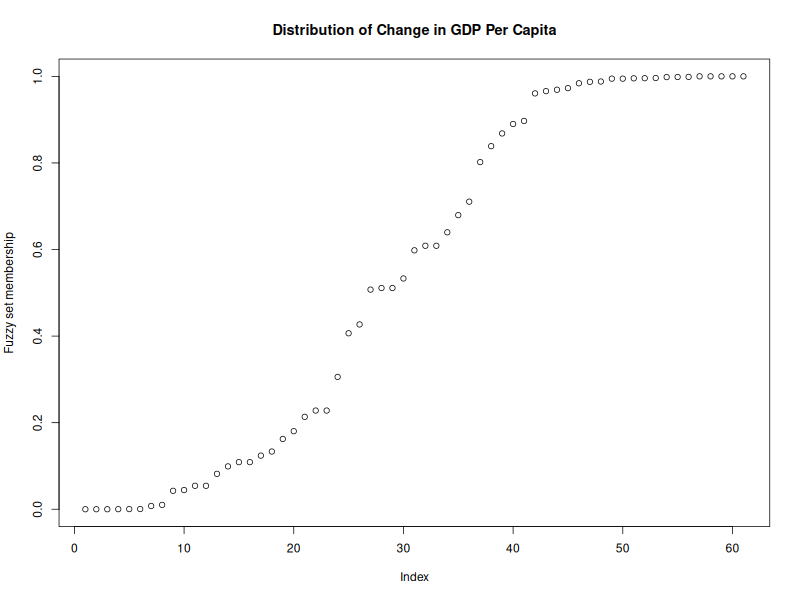
\includegraphics[width=\textwidth]{Graphics//calibration/gdppc_diff.png}
        \caption{Distribution of fuzzy-set scores for change in GDP per capita}
        \label{fig:gdppc}
    \end{minipage}
    \hfill
    \begin{minipage}{0.48\textwidth}
        \centering
        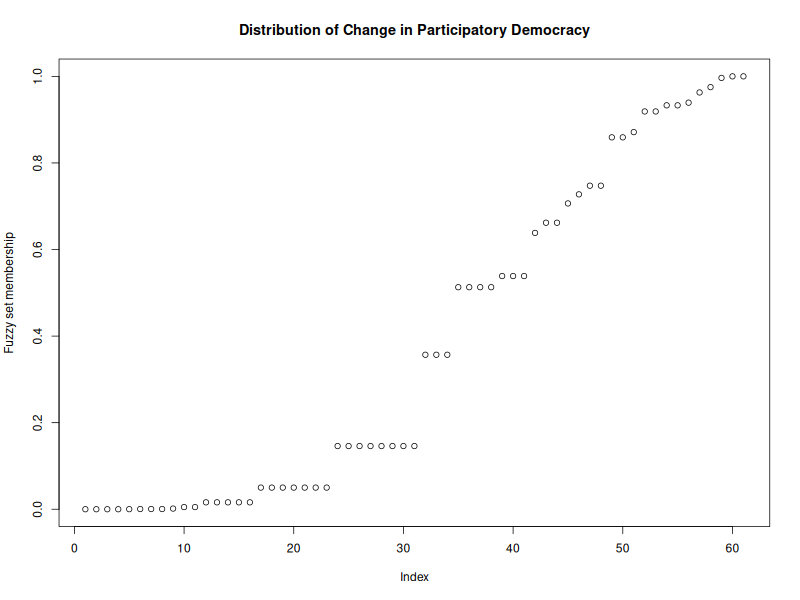
\includegraphics[width=\textwidth]{Graphics//calibration/partipdem.png}
        \caption{Distribution of fuzzy-set scores for change in participatory democracy}
        \label{fig:partipdem-dif}
    \end{minipage}
    \begin{minipage}{0.48\textwidth}
        \centering
        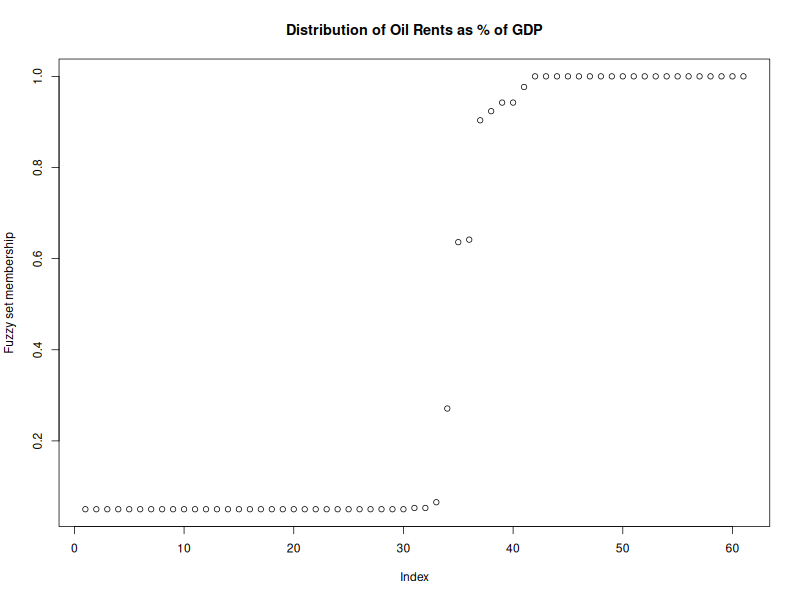
\includegraphics[width=\textwidth]{Graphics//calibration/oil_rents.png}
        \caption{Distribution of fuzzy-set scores for oil rents as \% of GDP}
        \label{fig:oil-rents}
    \end{minipage}
    \hfill
    \begin{minipage}{0.48\textwidth}
        \centering
        
\includegraphics[width=\textwidth]{Graphics//calibration/deaths.png}
        \caption{Distribution of fuzzy-set scores for fatalities}
        \label{fig:deaths}
    \end{minipage}
\end{figure}
\begin{figure}[ht]
    \centering
    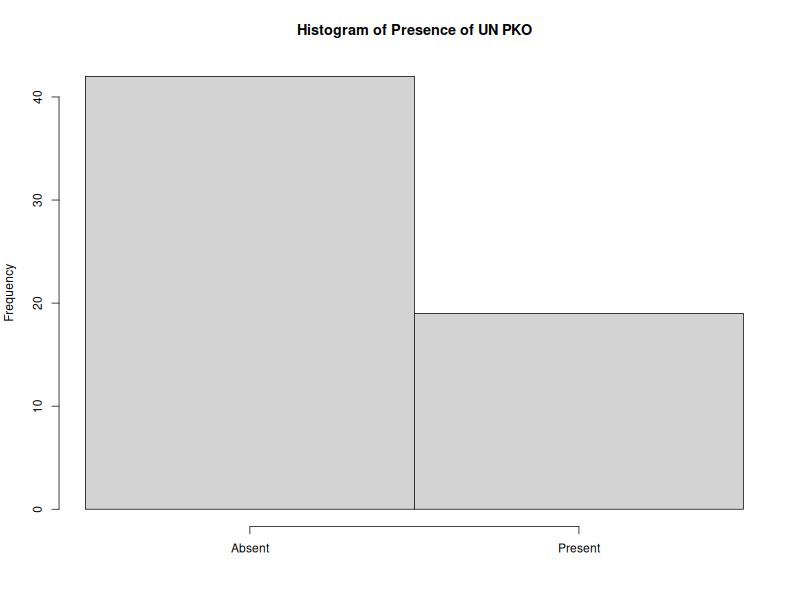
\includegraphics[width=\textwidth]{Graphics//calibration/un_pko.png}
    \caption{Distribution of crisp-set scores for presence or absence of UN PKO}
    \label{fig:un-pko}
\end{figure}
%Put data files, CAD drawings, additional sketches, etc.

\end{document}
